\chapter{Sequenzdiagramme}

\section{Import von einem JOANA Graphen}

\begin{figure}[!htbp]
  \centering
  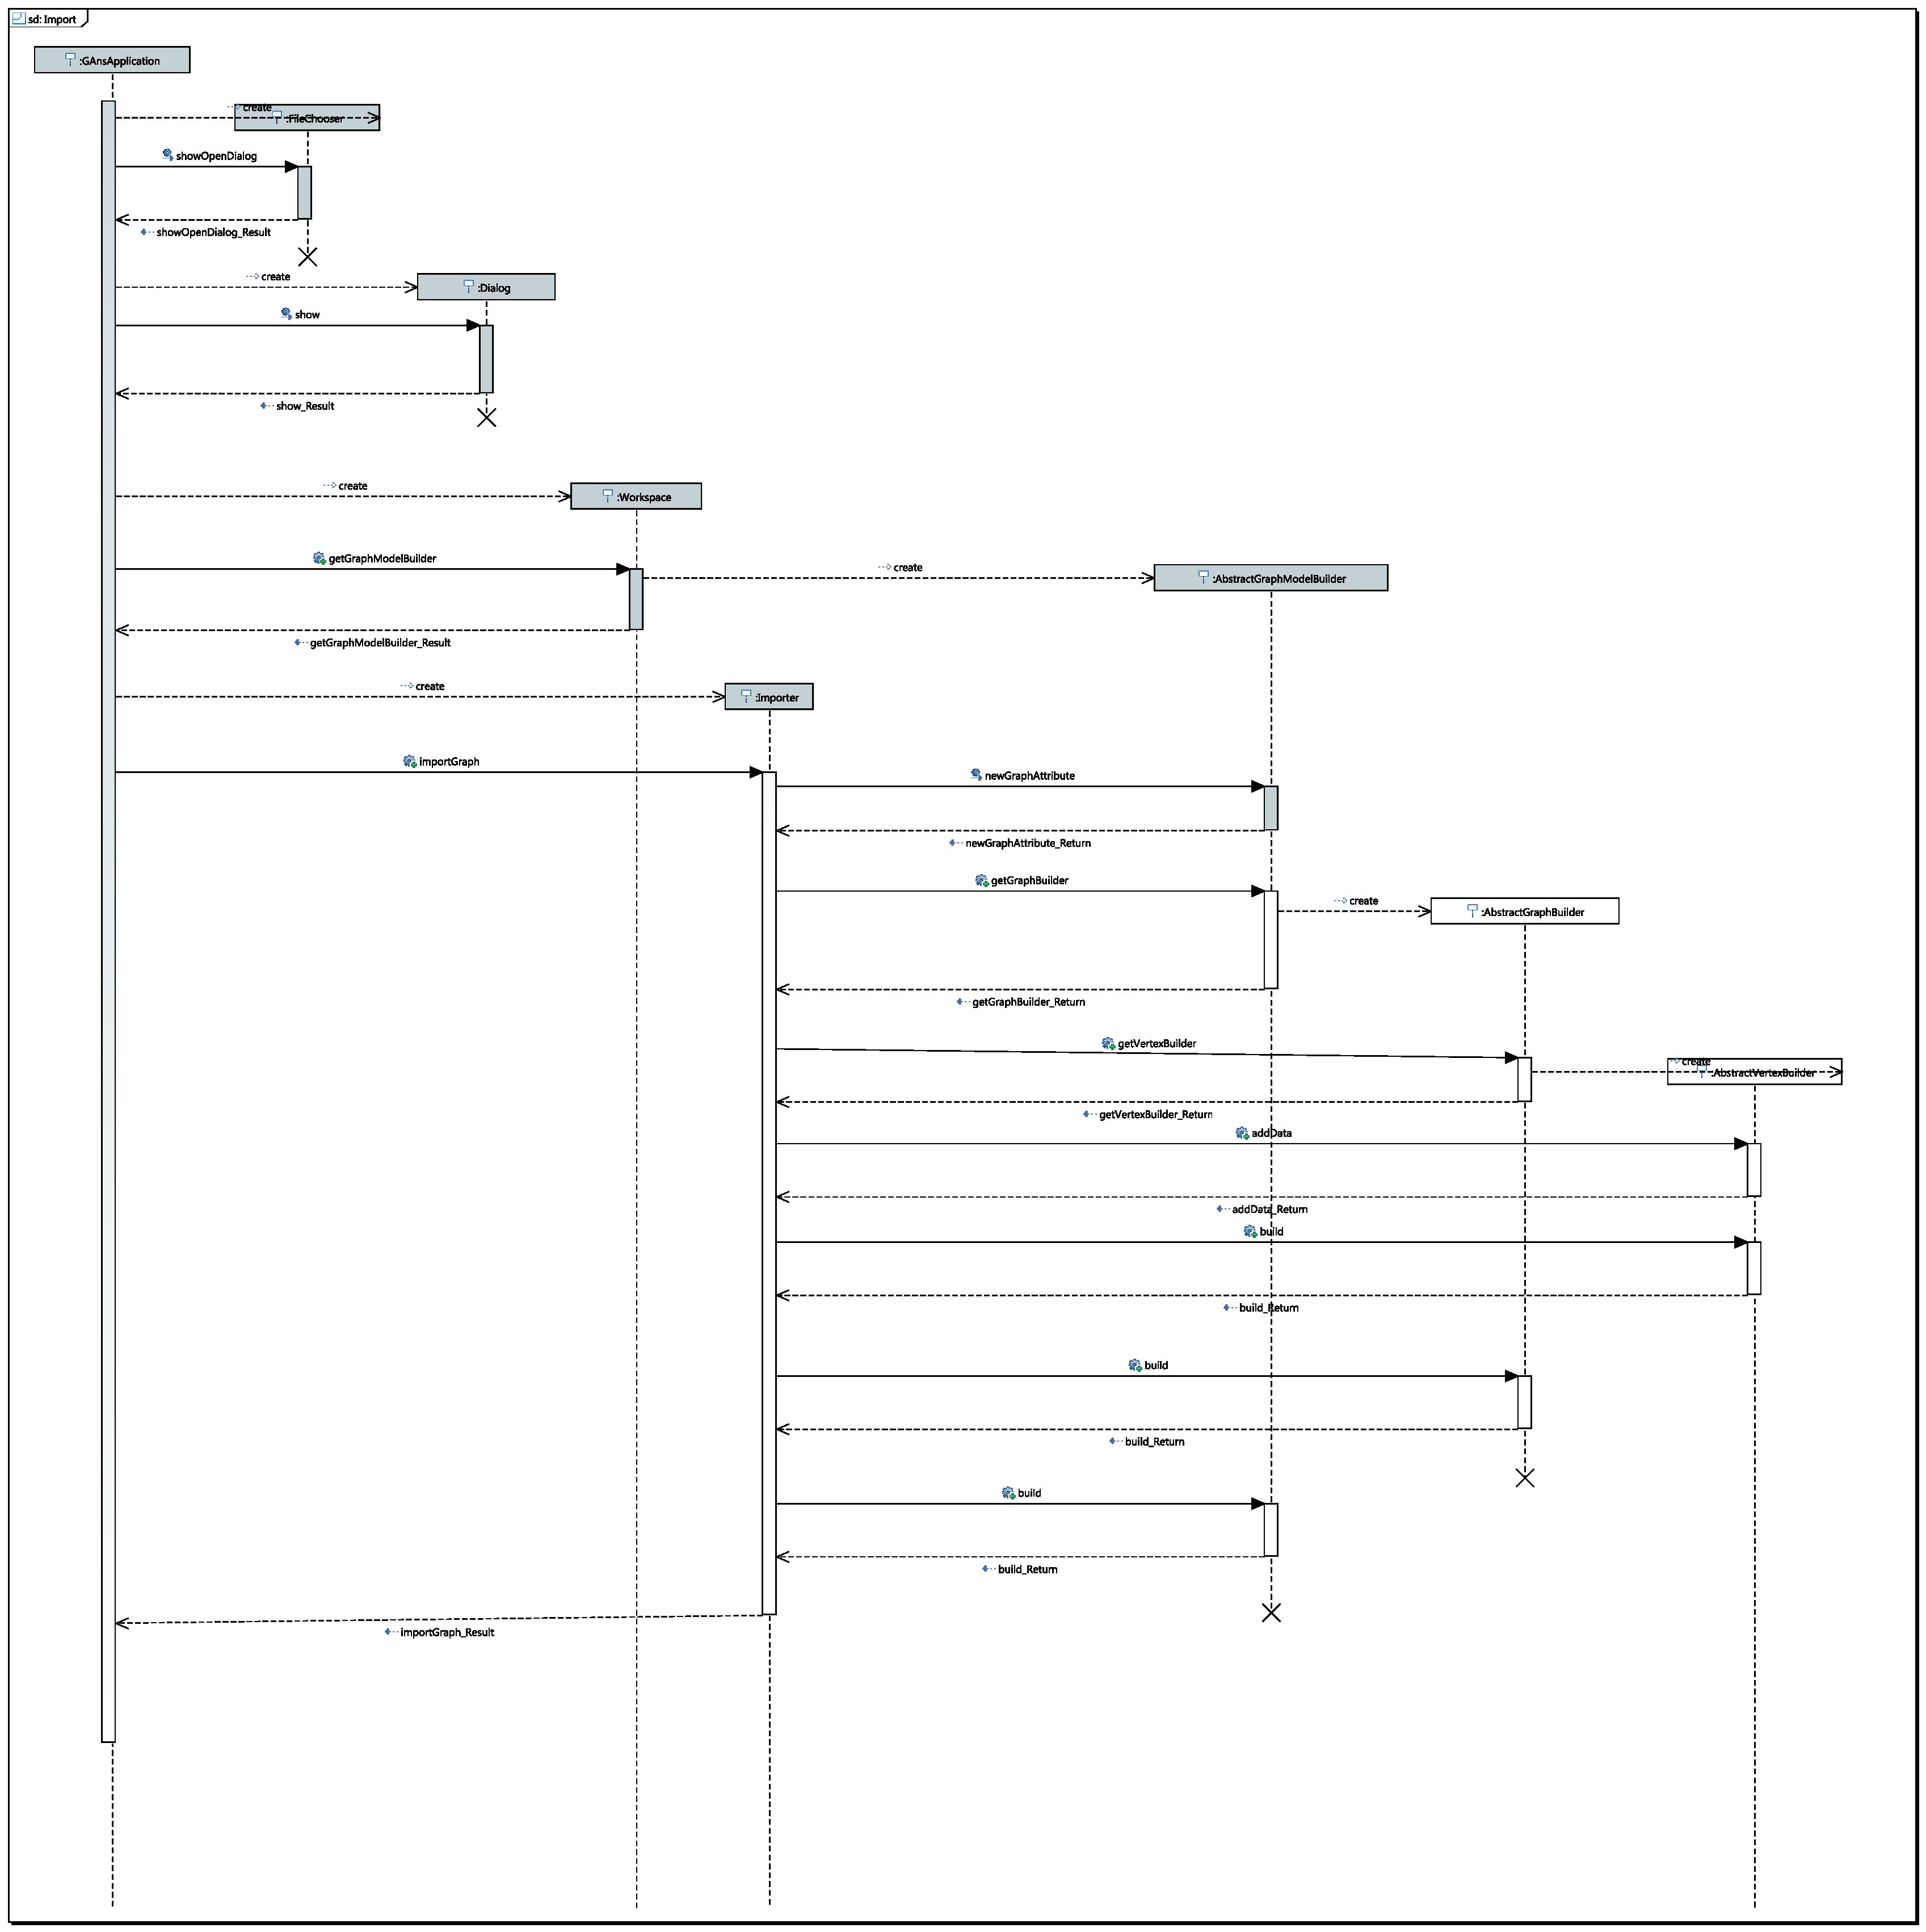
\includegraphics[width=450pt]{resourcen/SeqDiagramImport.PDF}
  \caption{Sequenz Diagramm für den Import}
  \label{fig:seq:import}
\end{figure}

Der Benutzer möchte einen Graphen importieren und klickt auf Import. Die GAnsApplication öffnet einen FileChooser, in welchem der Benutzer die Datei auswählen kann welche er importieren möchte. Danach öffnet sich ein Workspace Dialog in welchem der Benutzer auswählt als welcher Typ der Graph interpretiert werden soll.\\
Das Workspace übergibt der GAnsApplication nun den dazugehörigen IGraphModelBuilder. Dieser wird dann dem Importer übergeben, welcher mithilfe des Builders eine Repräsentation des Graphen erstellt, welche Workspace spezifisch ist.

\newpage

\section{Öffnen eines Graphen über die Strukturansicht}

\begin{figure}[!htbp]
	\centering
	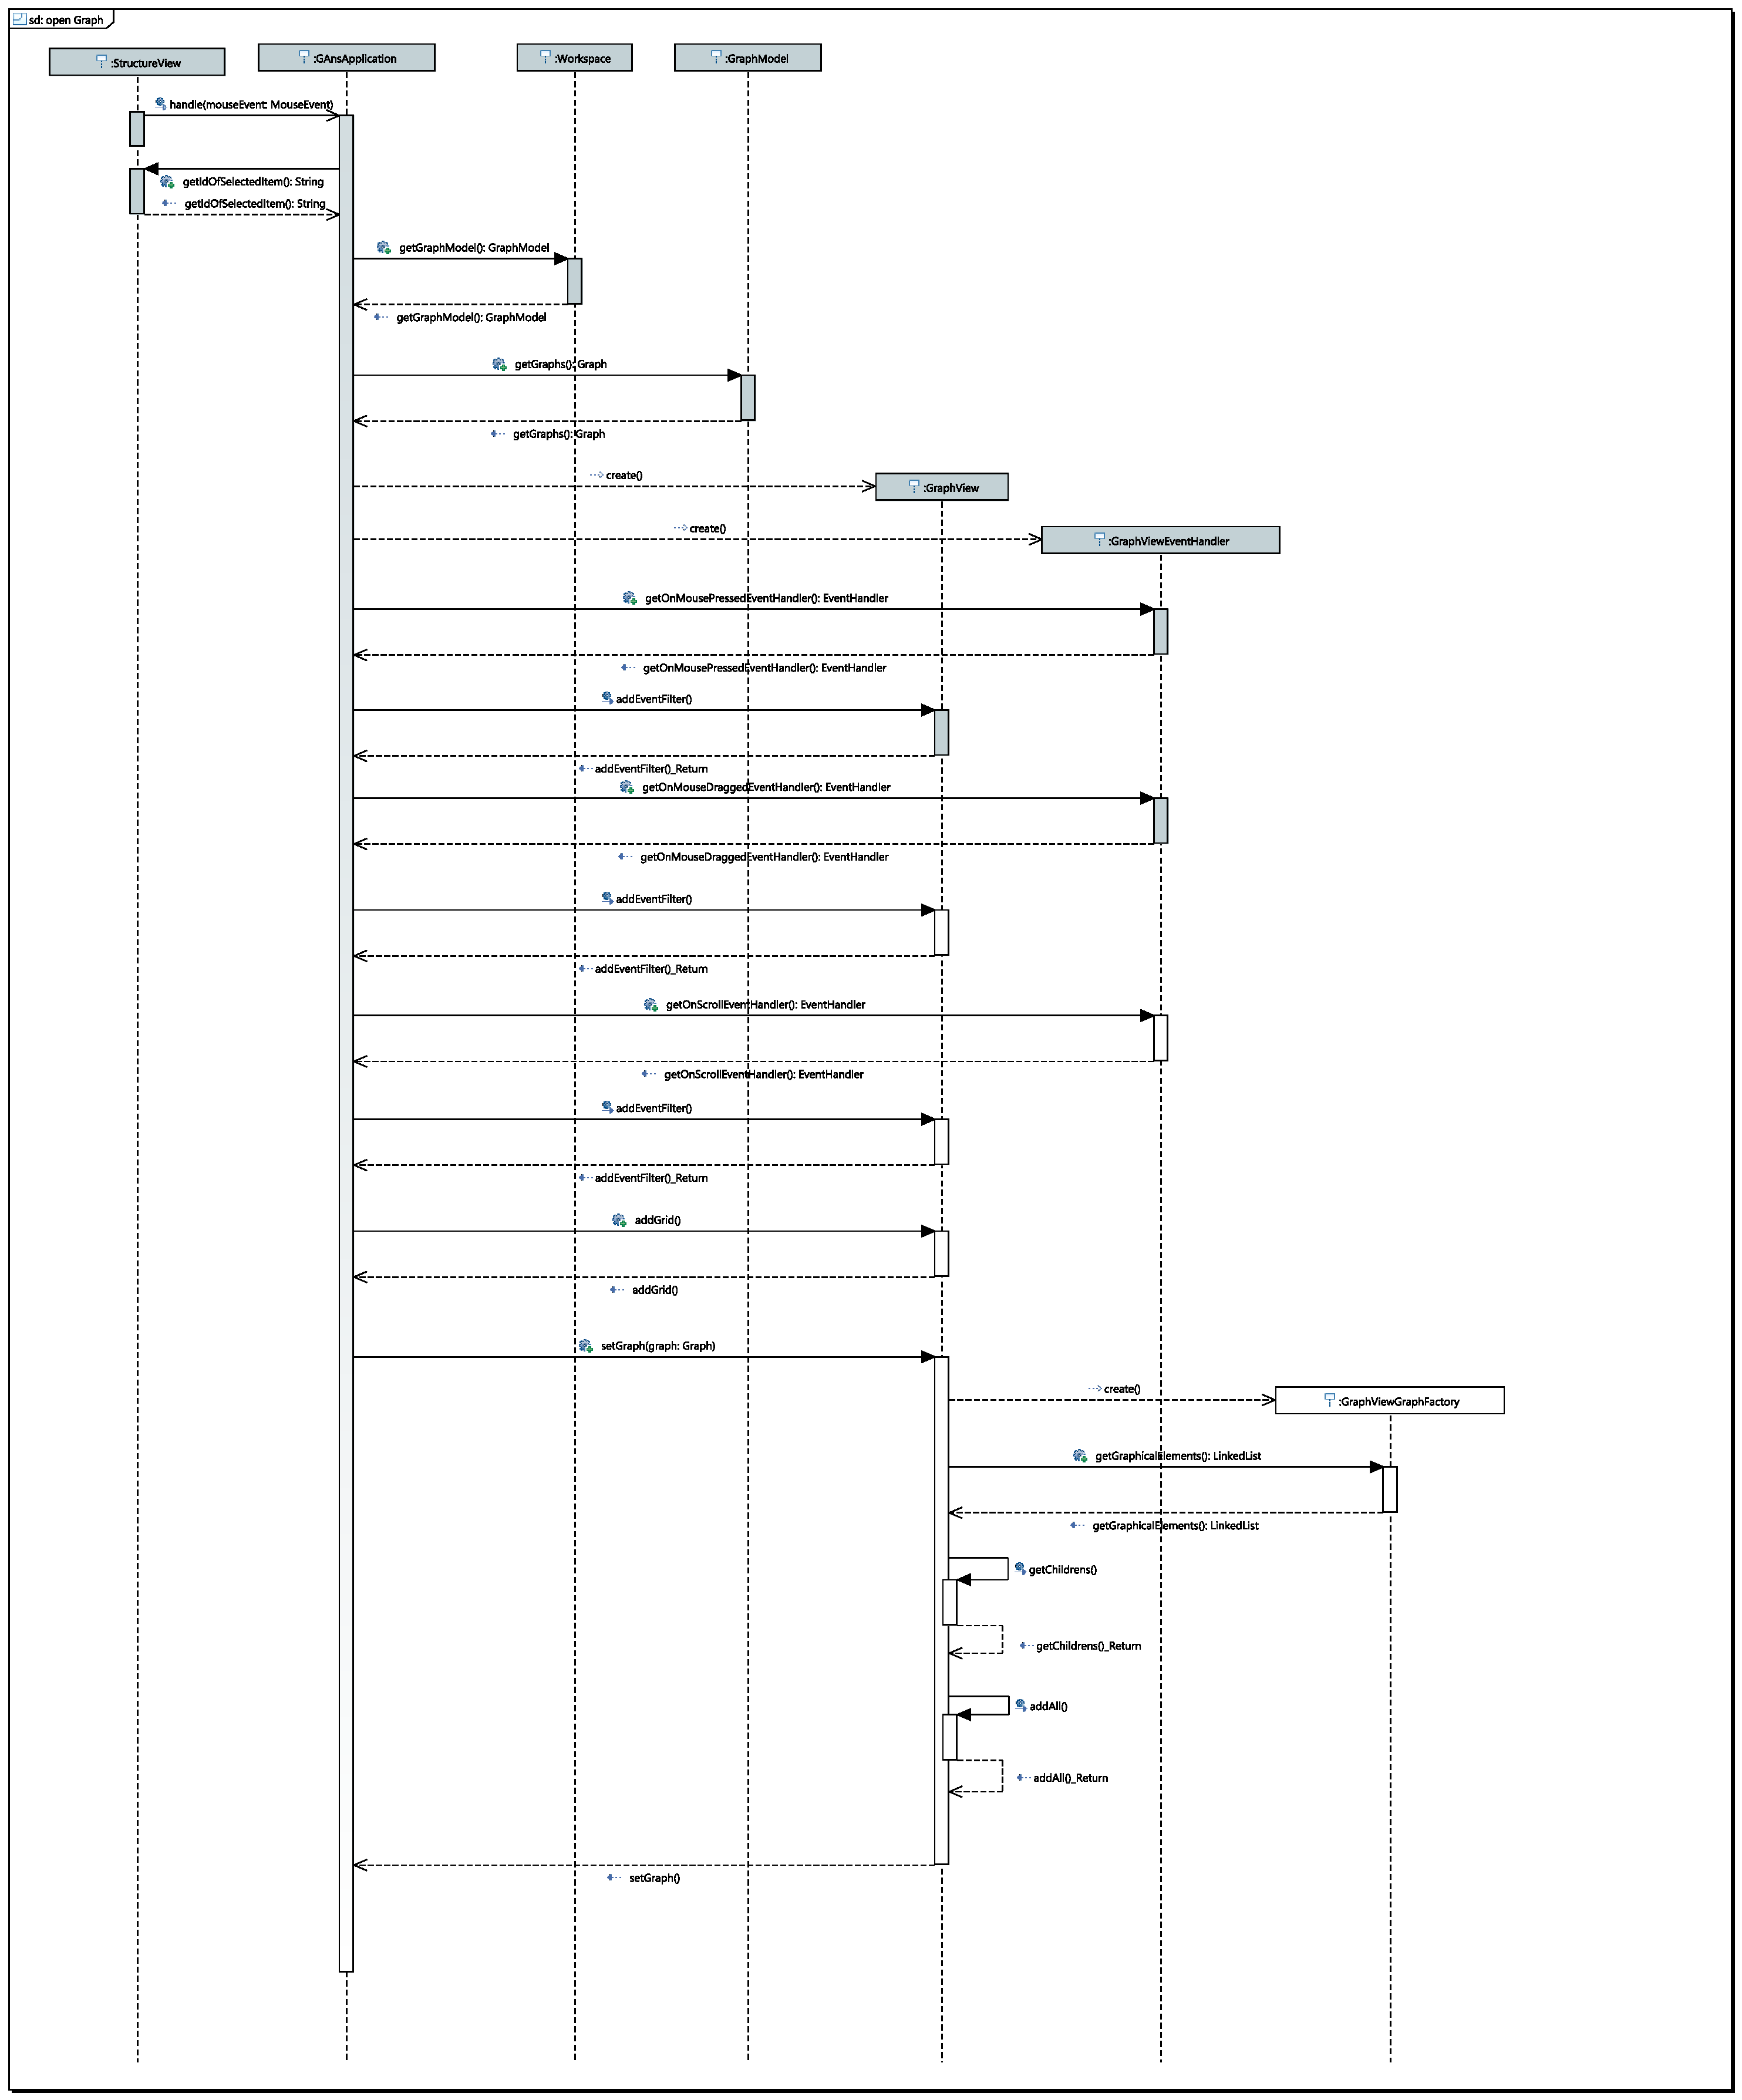
\includegraphics[width=450pt]{resourcen/SeqDiagramOpenGraph.PDF}
	\caption{Sequenz Diagramm das Öffnen eines Graphen aus der Strukturansicht}
	\label{fig:seq:openMethod}
\end{figure}

Der Benutzer hat einen Doppelklick auf ein Element in der StruktureView gemacht. Aus der StruktureView wird die ID des selektierten, gerade doppelt angeklickten, Elements gespeichert. Über das Workspace wird in den Graphen des geladenen GraphModels nach dem zur ID gehörenden Graph gesucht. Der gefundene Graph wird nun gelayouted (siehe \ref{fig:seq:layout}) dabei werden nicht die Dialoge geöffnet, sondern direkt die default LayoutOption des Workspace für den Graphen verwendet. Nachdem der Graph vom layouten zurückgegeben wird, wird eine neue GraphView und ein neues GraphViewEventHandler-Objekt erzeugt, die einzelnen EventFilter werden zur GraphView hinzugefügt und ein Grid wird gesetzt, welches für die Zoom-Funktion benötigt wird. Ist die GraphView aufgesetzt, wird der Graph an sie übergeben. Die GraphView erzeugt eine eigene Factory, welche passend zum Graphen, GraphischeElemente erzeugt. Die GraphView setzt diese Elemente, wodurch sie angezeigt werden.

\newpage

\section{Ändern der Selektion im Graphen}

\begin{figure}[!htbp]
	\centering
	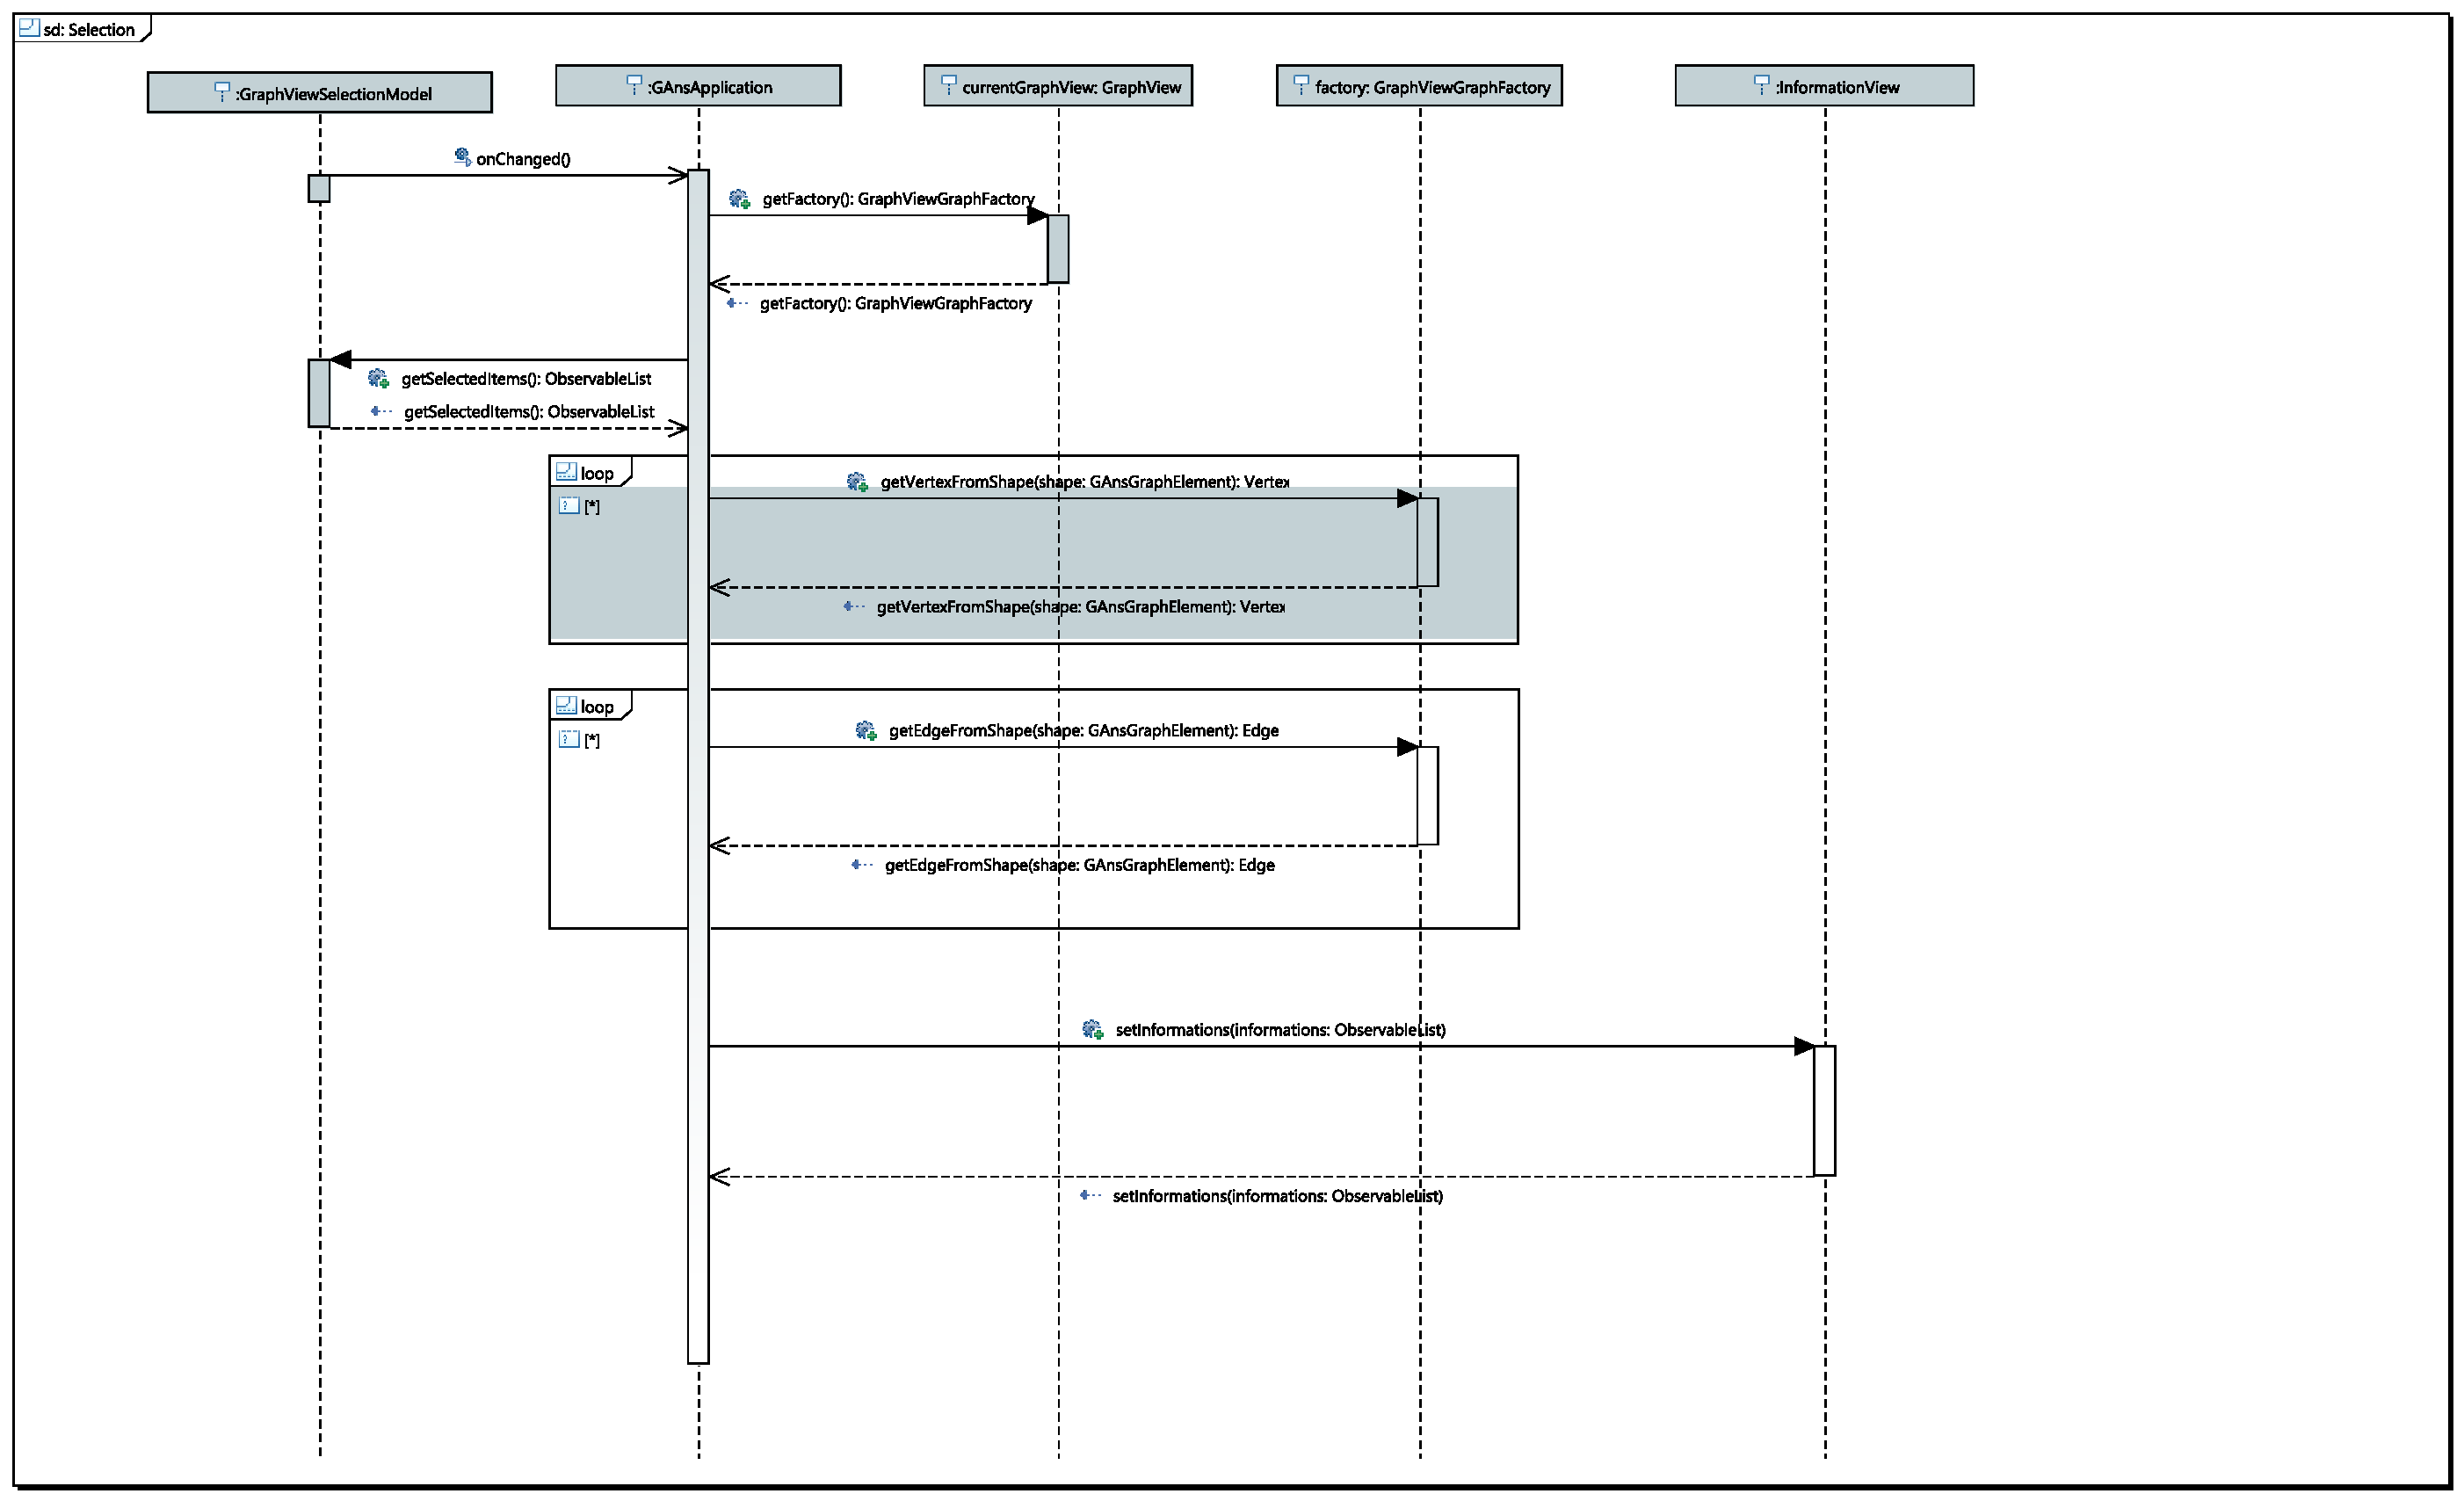
\includegraphics[width=450pt]{resourcen/SeqDiagramSelection.PDF}
	\caption{Sequenz Diagramm für geänderte Selektion}
	\label{fig:seq:selection}
\end{figure}

Der Benutzer hat in der aktuellen GraphAnsicht die Selektion geändert. Die GAnsApplication wird vom GraphViewSelectionModel benachrichtigt. Die GAnsApplication holt sich von der aktuellen GraphAnsicht die Factory, welche zugriff auf die Elemente in der GraphView bietet, und vom SelectionModel eine Liste mit allen selektierten Elementen. Über die Factory und wird nun zu jedem selektiertem Element die zugehörige Vertex oder Edge aus dem angezeigten Graphen ermittelt. Deren GAnsProperties werden in eine ObservableList zusammengeführt und an die InformationsView übergeben, welche die Informationen die über die Properties gegeben sind darstellt.

\newpage

\section{Layouten eines JOANA-Graphs}

\begin{figure}[!htbp]
	\centering
	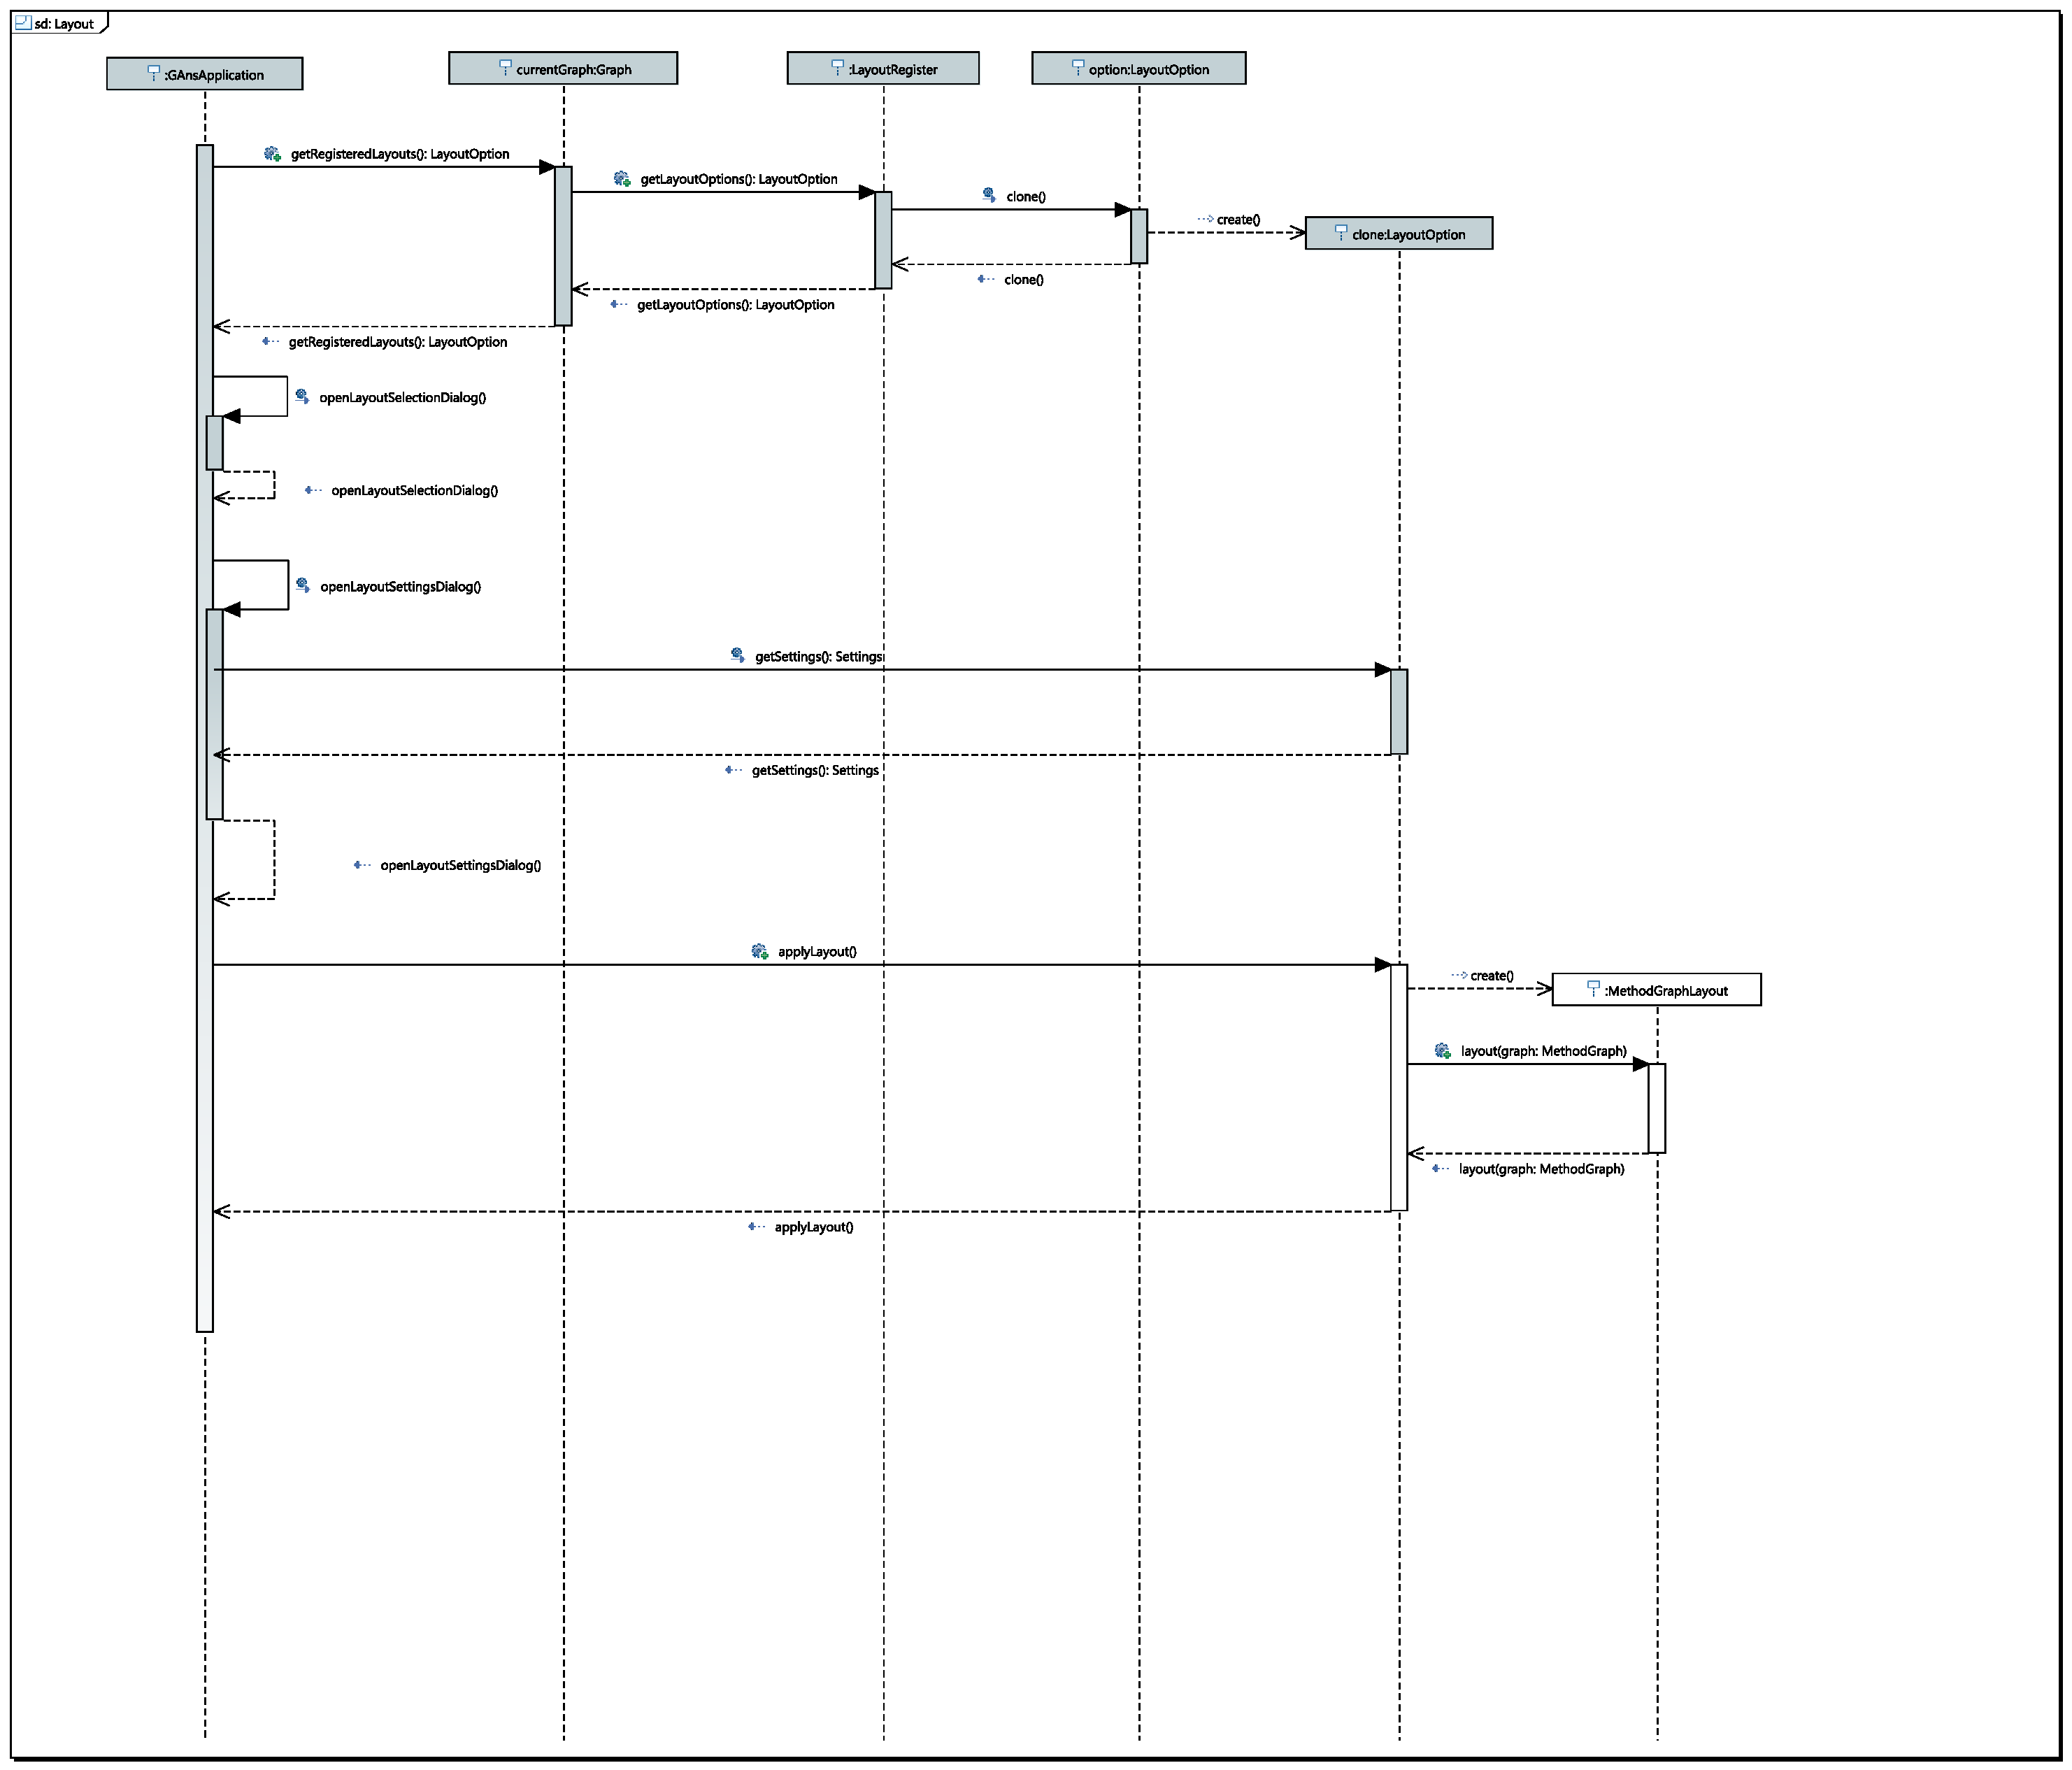
\includegraphics[width=450pt]{resourcen/SeqDiagramLayout.PDF}
	\caption{Sequenz Diagramm für Layouten eines JOANA-Graphs, Oberfläche}
	\label{fig:seq:layout}
\end{figure}

Der Benutzer hat das Layouten des angezeigten Graphen über einen Menüeintrag angestoßen. Die GAnsApplication holt sich über den Graphen alle registrierten LayoutOptions. Diese werden in einem Dialog zur Auswahl gestellt. Nachdem der Benutzer eine Wahl getroffen hat wird ein Dialog geöffnet in dem Einstellungen zur gewählten LayoutOption gemacht werden können. Nun wird auf den gewählten LayoutOption applyLayout aufgerufen, ein MethodGraphLayout erstellt und auf den Graph angewendet(siehe \ref{fig:seq:layoutSugi}).
\newpage

\begin{figure}[!htbp]
	\centering
	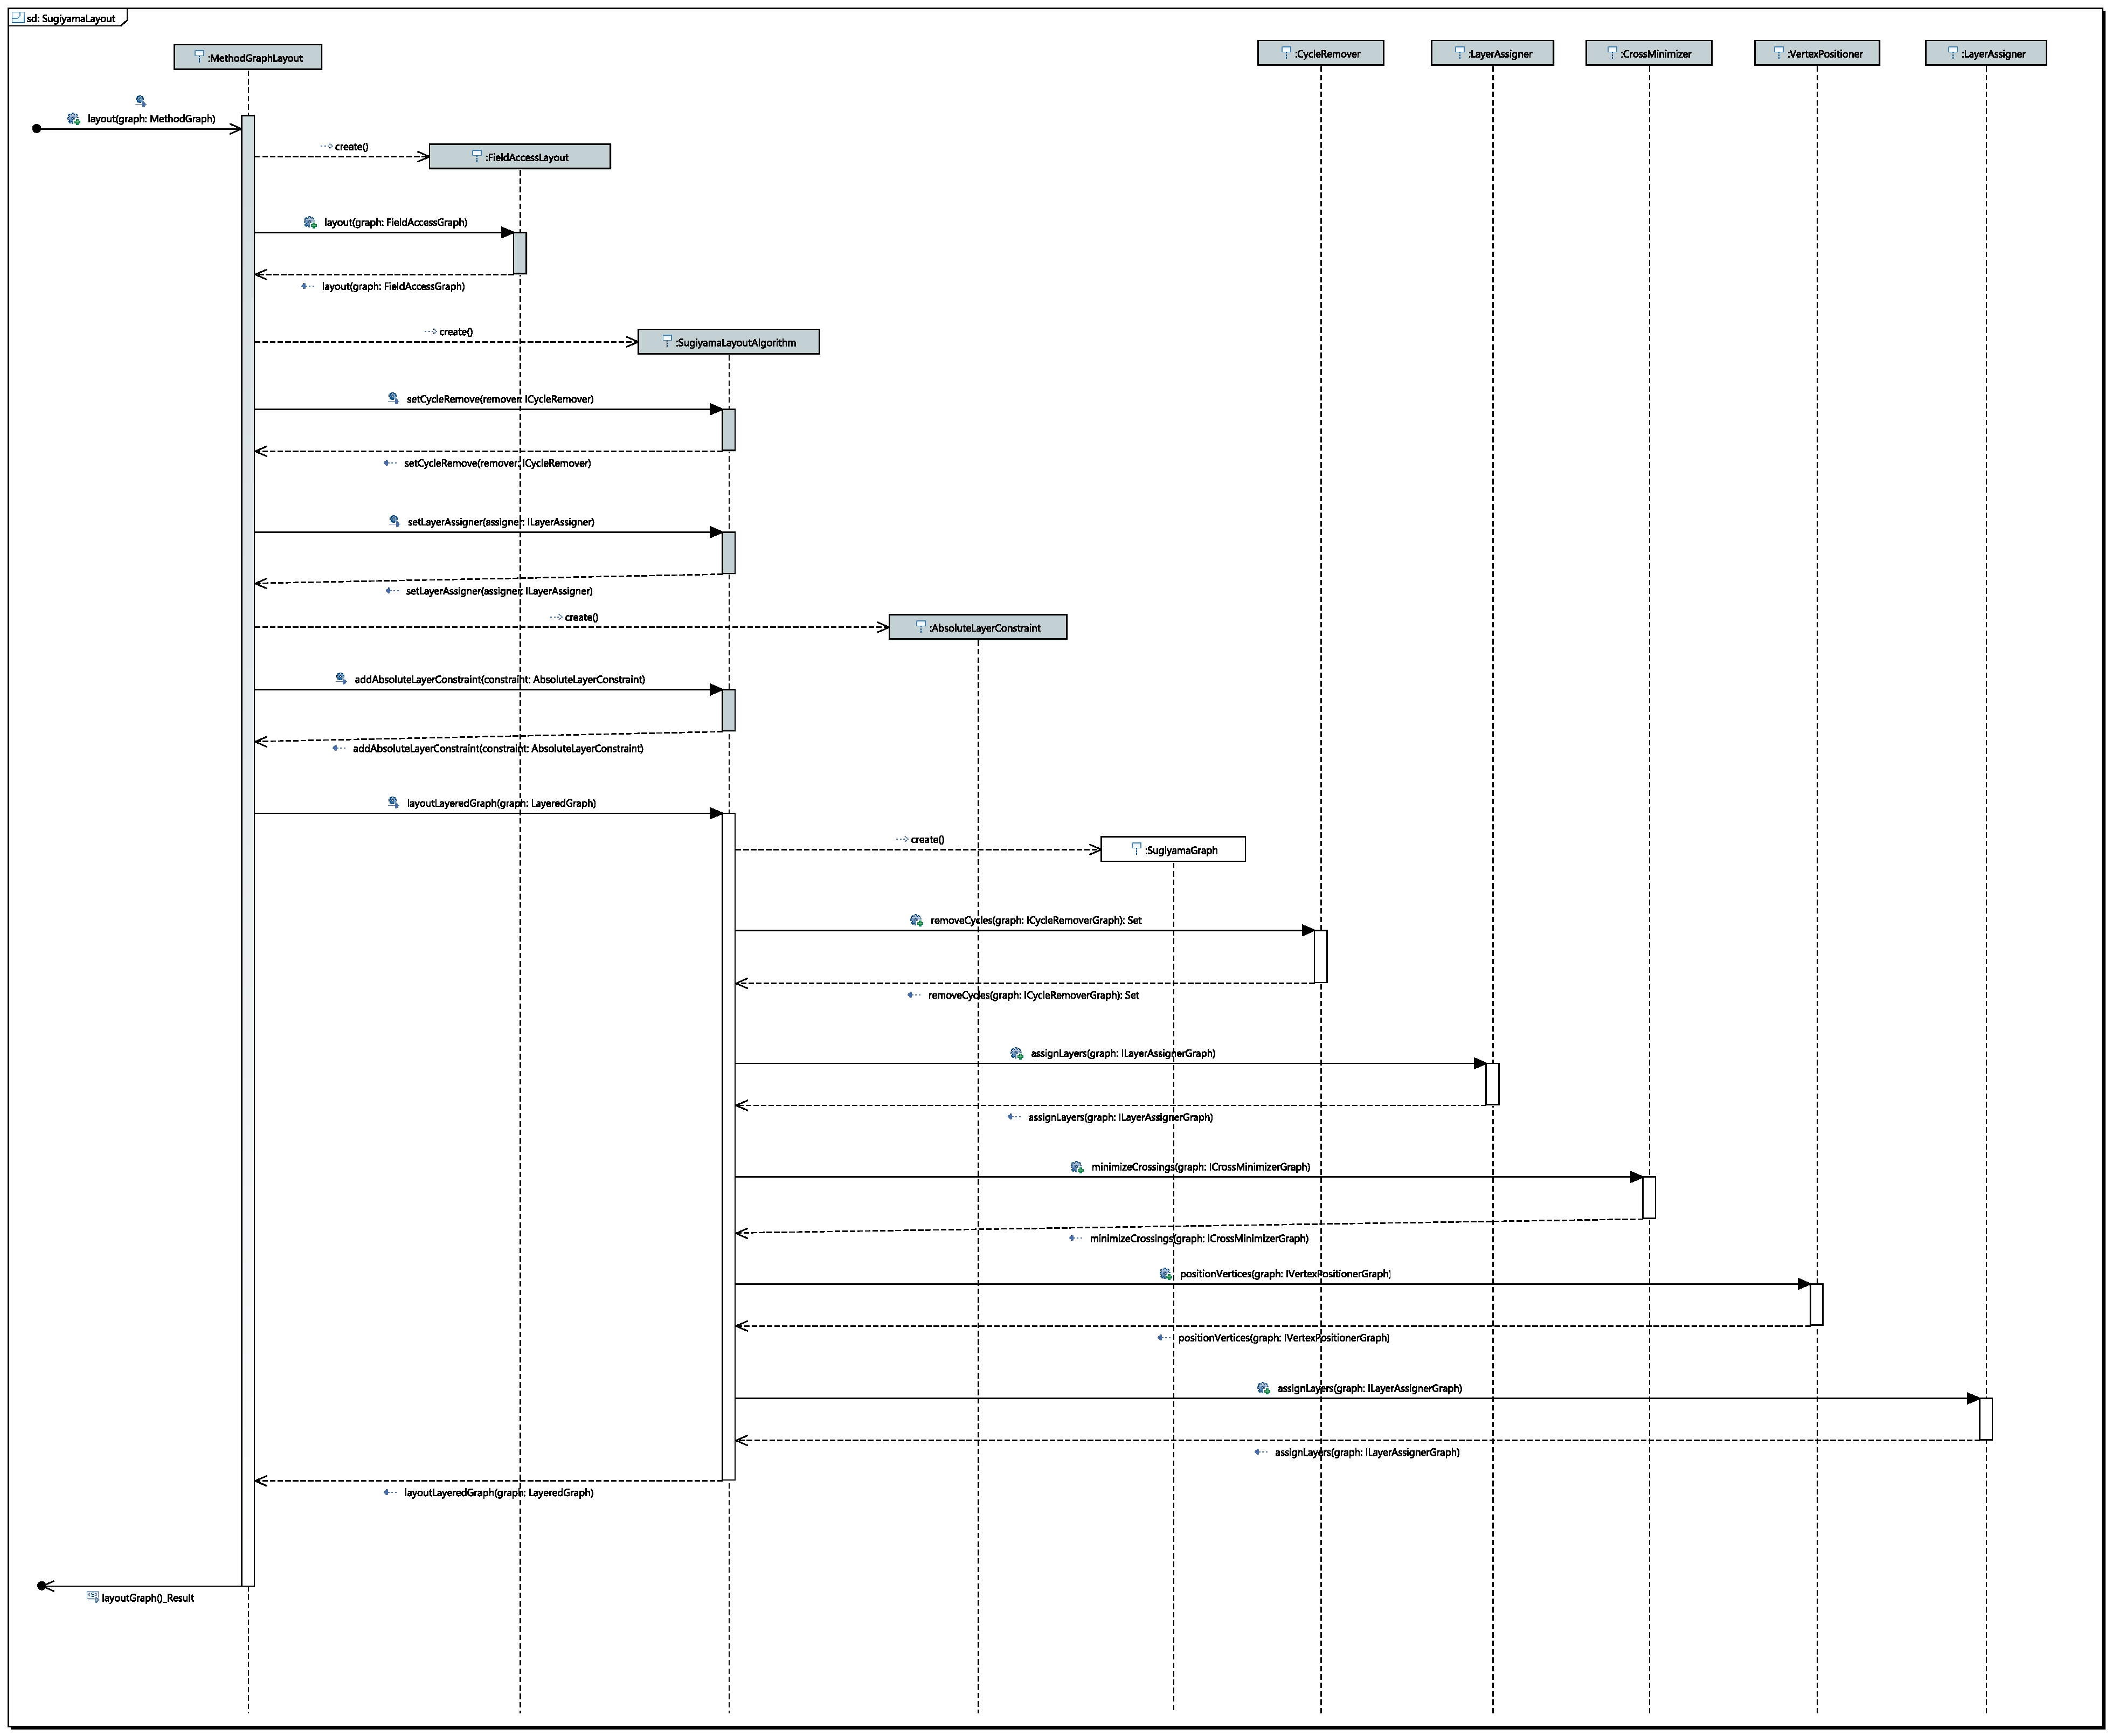
\includegraphics[width=450pt]{resourcen/SeqDiagramSugiyama.PDF}
	\caption{Sequenz Diagramm für Layouten eines JOANA-Graphs, Sugiyama}
	\label{fig:seq:layoutSugi}
\end{figure}

Nachdem das Layouten mit dem MethodGraphLayout angestoßen wurde, wird zuerst ein FieldAccessLayout erstellt und damit alle FieldAccessGraphen des MethodenGraphen gelayouted. Danach wird ein SugiymaLayoutAlgorithm erstellt, die jeweiligen Phasen gesetzt, ein SugiyamaGraph erstellt und die jeweiligen Phasen auf den Graphen angewandt.

\newpage
\section{Export von einem geladenen JOANA-Graphen als SVG}

\begin{figure}[!htbp]
	\centering
	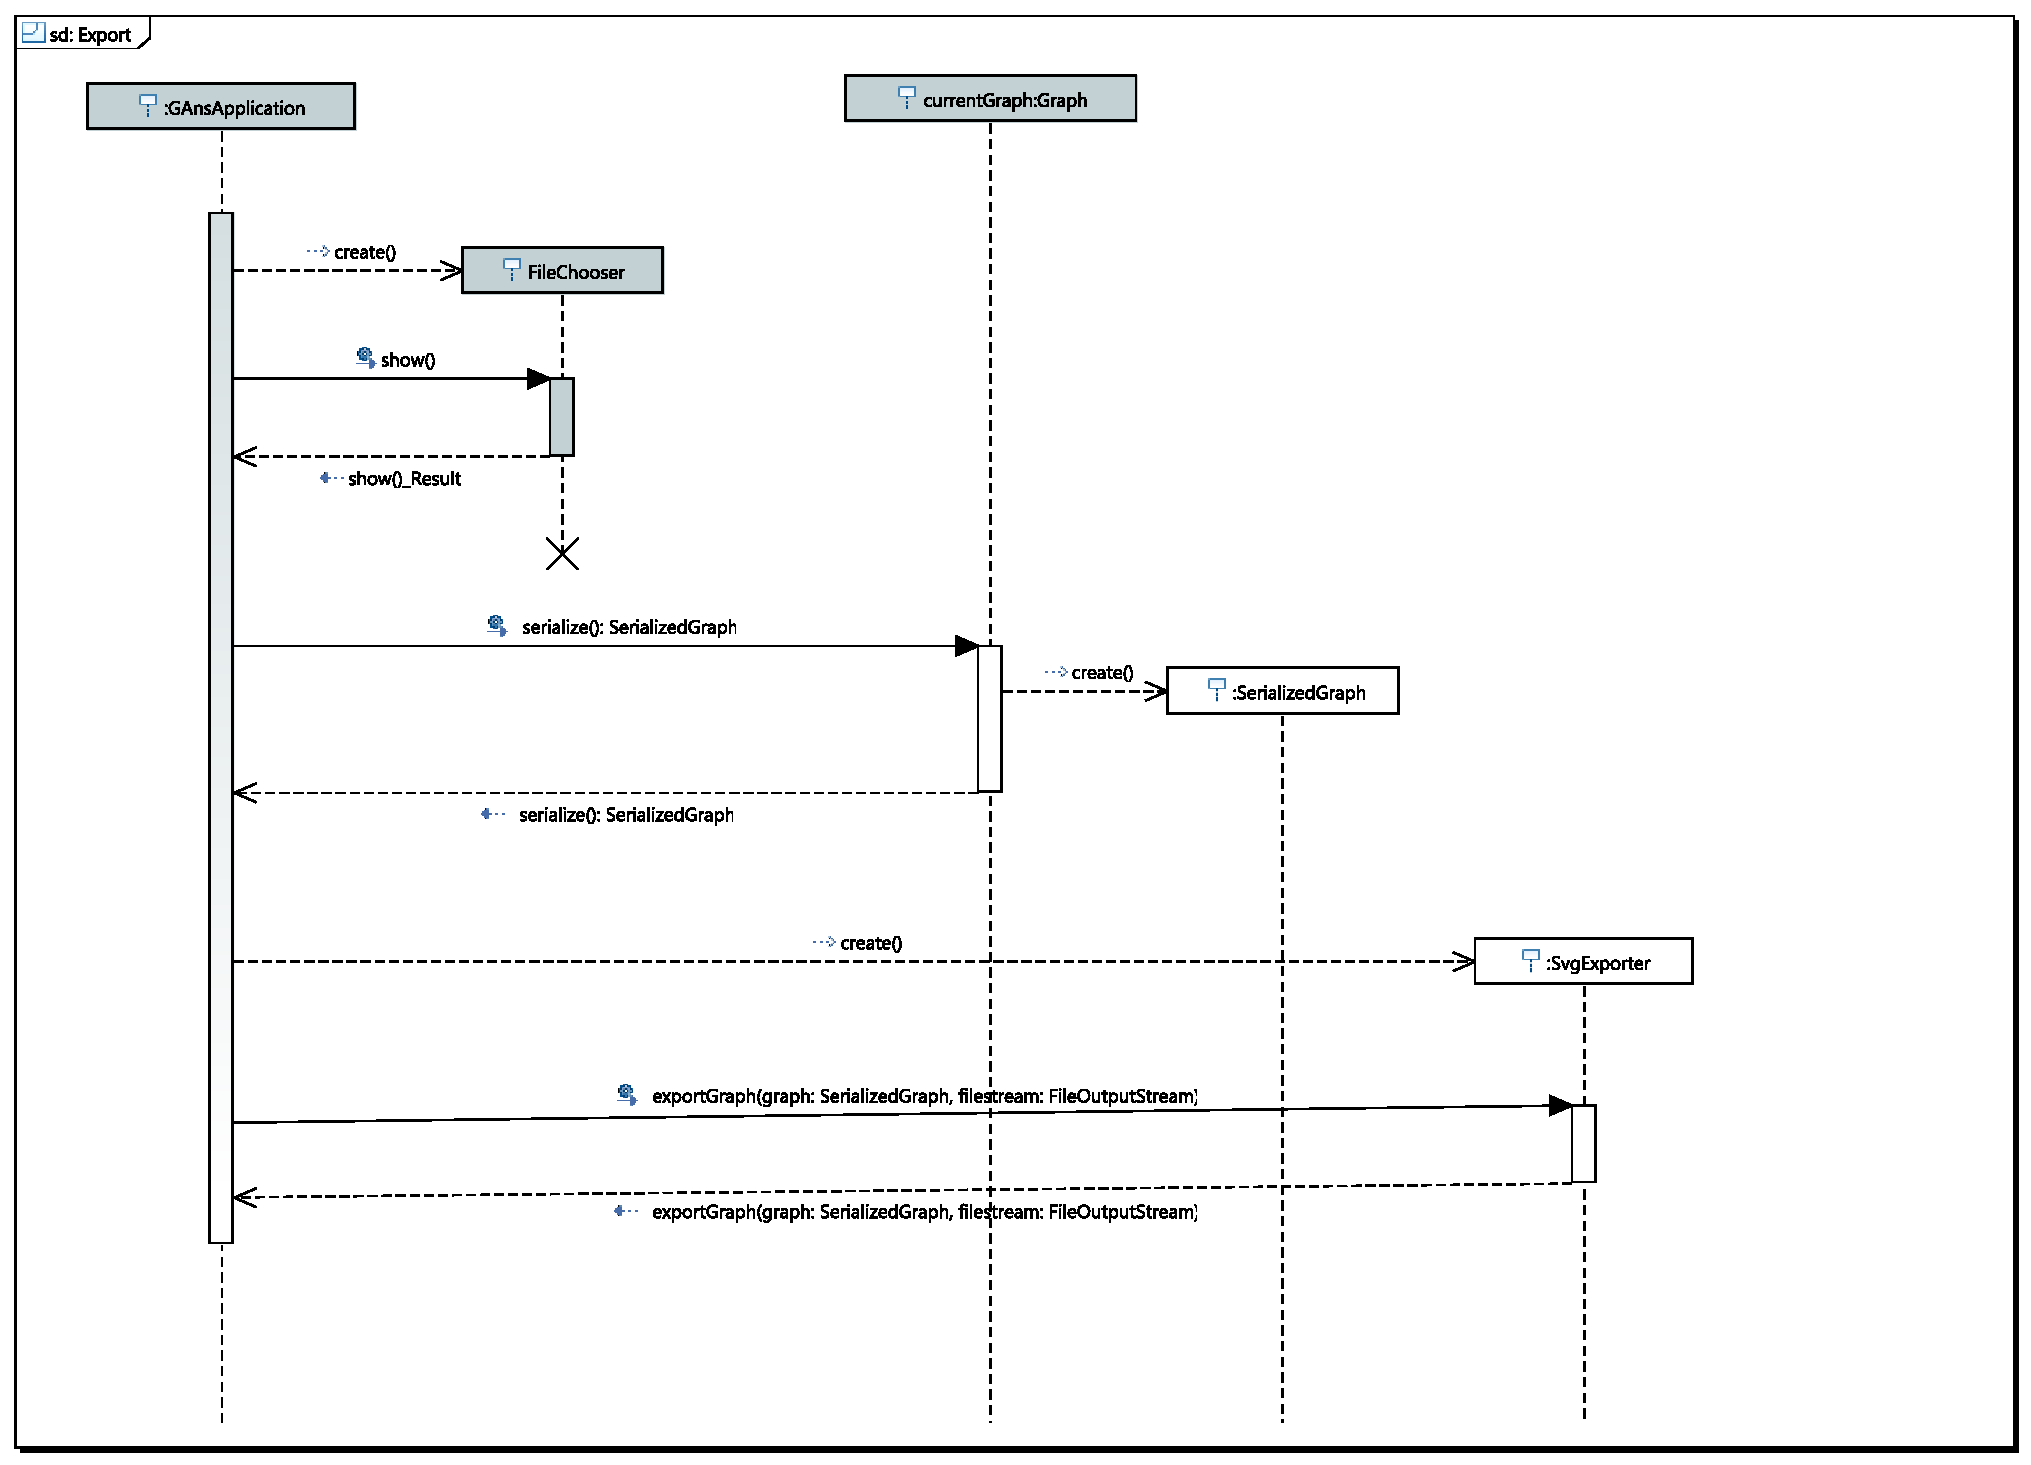
\includegraphics[width=450pt]{resourcen/SeqDiagramExport.PDF}
	\caption{Sequenz Diagramm für Layouten eines JOANA-Graphs, Sugiyama}
	\label{fig:seq:export}
\end{figure}

Der Benutzer möchte einen Graphen exportierten und klickt auf Export. Die GAnsApplication öffnet einen FileChooser, in welchem der Benutzer den Ort und Namen der Datei angeben kann, in die exportiert werden soll. Danach wird der Graph serialisiert und dessen serialisierte Repräsentation in den SvgExporter gegeben, welcher die Daten aus dem Graph in SVG-Form an den ausgewählten Ort schreibt.